\section{Training Results}
\label{sec:results}

\Cref{tab:results} lists the final held-out success of every method together with paired comparisons
against both controls, and \cref{fig:curves} shows the learning curves.

\begin{table}[t]
\centering\footnotesize
\setlength{\tabcolsep}{3.2pt}
\begin{tabular}{@{}lrrcc@{}}
\toprule
Method & Final & Best & vs.\ GRPO & vs.\ GACA \\
\midrule
Base model (no training) & 4.7 & -- & -- & -- \\
GRPO~\cite{shao2024deepseekmath} & 14.1 & 14.1 & -- & 13/7 (0.26) \\
GACA~\cite{liang2026gaca} & 18.8 & 18.8 & 7/13 (0.26) & -- \\
\midrule
GACA + $m_z$ gate & 12.5 & 12.5 & 13/11 (0.84) & 17/9 (0.17) \\
GACA-LOO (App.~B.4 of~\cite{liang2026gaca}) & 11.7 & 11.7 & 11/8 (0.65) & 14/5 (0.064) \\
\textbf{COMMIT (ours)} & 20.3 & 20.3 & 8/16 (0.15) & 14/16 (0.86) \\
\quad clip $[0.5, 2]$ & 14.1 & 14.1 & 13/13 (1.00) & 16/10 (0.33) \\
\quad positive $A_t$ only & 5.5 & 6.2 & \textbf{16/5 (0.027)} & \textbf{20/3 (<0.001)} \\
\bottomrule
\end{tabular}

\caption{\textbf{Held-out success (\%) on the same 128 ALFWorld games}, 34 training iterations
(33 for the two GACA step variants), one seed per method. \emph{Final} is the end-of-training
checkpoint, \emph{Best} the maximum over five evaluations. The comparison columns give $b/c$
(McNemar $p$): $b$ games solved only by the control, $c$ only by the method in that row; bold
$p < 0.05$.}
\label{tab:results}
\end{table}

\begin{figure}[t]
\centering
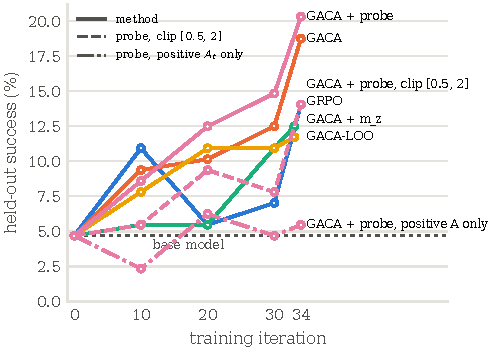
\includegraphics[width=\linewidth]{figs/curves.pdf}
\caption{\textbf{Held-out success over training} (128 games, evaluated every 10 iterations). Colour
follows the method; variants of the probe keep its colour and change line style.}
\label{fig:curves}
\end{figure}

\paragraph{Controls.}
Both controls learn: GRPO reaches 14.1\% and GACA 18.8\% from the base model's 4.7\% (both $p < 0.05$
against the base model, game-paired). GACA leads GRPO by 13 games to 7
($p = 0.26$): at this budget the ordering is not resolved. GACA's gate is active in our runs: the
criticality score has standard deviation 0.35 and $\lambda_t$ has standard deviation 0.087, so steps do
receive different mixtures.

\paragraph{Probe-weighted token credit.}
GACA + probe reaches 20.3\%, the highest final success of any method, after rising at every evaluation
(4.7, 8.6, 12.5, 14.8, 20.3) and leading every arm from iteration 20 on. It also has the highest
training-batch success (11.2\% averaged over iterations, against 9.2\% for GACA). Game by game it solves
16 games GACA misses while missing 14 that GACA solves ($p = 0.86$), and against GRPO the split is 16 to
8 ($p = 0.15$). We read this as \emph{consistent with} a benefit, not as evidence for one: with one seed
per arm and a 3-point seed-to-seed spread observed earlier, a 1.5-point lead over GACA is well within
noise. The probe's cost is visible in wall-clock: 550\,s per iteration against 389\,s for GACA, of which
151\,s is the probe passes. Its updates are moderately larger than GACA's (mean gradient norm 1.06
against 0.84, KL 0.024 against 0.020), as expected when the same advantage is concentrated on fewer
tokens. The probability of the eventual action before any reasoning, $q(0)$, \emph{fell} from 0.19 to
0.14 over training, so the reasoning became more causally important rather than decorative, the
opposite of the drift Yu~\etal~\cite{yu2026cir} warn about for outcome rewards.

\paragraph{How the probe is applied matters.}
The two variants were designed to fix failure modes of concentration, and none helped.
A tighter clip $[0.5, 2]$ brought the gradient norm to GACA's level (0.93) and finished at 14.1\%, level
with GRPO. Applying the probe only to positive advantages, so that blame always stays uniform, was the
worst method: 5.5\%, essentially no learning, and significantly below both GRPO (16 to 5, $p = 0.027$)
and GACA (20 to 3, $p < 0.001$). Its KL rose to 0.059 over the last iterations although $q(0)$ stayed flat
(0.20 to 0.19), so early commitment does not explain the failure. A plausible reading is that the
asymmetry itself is harmful: positive steps push hard on a few decisive tokens while negative steps push
weakly on all tokens, so the policy is moved toward specific reasoning patterns without a matching
signal moving it away from bad ones.

\paragraph{Step-level treatments.}
Neither change to GACA's step estimator helped. Scaling the gate's odds by $1 - 1/m_z$ changes little
because 96\% of steps already fall in anchor groups with $m_z \geq 2$; it finished at 12.5\%. The
leave-one-out score of GACA's Appendix B.4, which averages away the within-state noise we measured,
finished at 11.7\% and trails GACA by 14 games to 5 ($p = 0.064$). Pooling the score also shrinks the
spread of $\lambda_t$ to 0.039 from 0.087, so the gate barely adapts; in the paper's terms, it trades the
noise of the single-sample score for the loss of within-group resolution, and at this budget the trade
does not pay.
